

\chapter{VSNLib}                %crea il capitolo
%%%%%%%%%%%%%%%%%%%%%%%%%%%%%%%%%%%%%%%%%imposta l'intestazione di pagina
\lhead[\fancyplain{}{\bfseries\thepage}]{\fancyplain{}{\bfseries\rightmark}}
Interfaccia di configurazione degli stack di rete attraverso l'utilizzo di tecnologia netlink.
\section{Il Progetto}                 %crea la sezione
Gli stack analizzati in precedenza offrono a grandi linee la stessa tipologia di servizio seppur ognuna con le proprie caratteristice.\\
Nessuno dei progetti ha per\`o tenuto in considerazione l'idea di utilizzare un'interfaccia di configurazione che fosse standard, \`e pertanto necessario usare le funzioni specifiche per ognuno di questi progetti, costringendo il programmatore a cambiare modalit\`a di interazione da stack a stack.\\
L'idea di creare questa libreria nasce proprio dall' esigenza di uniformare le interfacce di comunicazione in modo tale che l'utente non sia costretto ad adattarsi ogni qual volta decida di cambiare stack.\\
\section{VSNLib}
\subsection{Preambolo}
Per configurare uno stack di rete programmi come {\tt {ip}}\footnote{il programma usato per configurare lo stack di rete tramite comandi quali {\tt {ip addr...}, \tt {ip link...}, \tt {ip route...} ecc.}} generano un pacchetto netlink con le informazioni necessarie lo inviano al kernel che lo elabora, esegue le operazioni e genera un messaggio contenente un flag attraverso il quale viene comunicato il tipo di errore (0 in caso di successo). A questo messaggio \`e associato un payload di risposta generalmente usato per comporre un feedback da mostrare all'utente che sta interagendo con il programma, in figura \ref{fig:nlmserror} lo schema dell'header per il messaggio di risposta.\\
\begin{figure}[h]                       %crea l'ambiente figura; [h] sta
                                        %   per here, cio� la figura va qui
\begin{center}                          %centra nel mezzo della pagina
                                        %   la figura
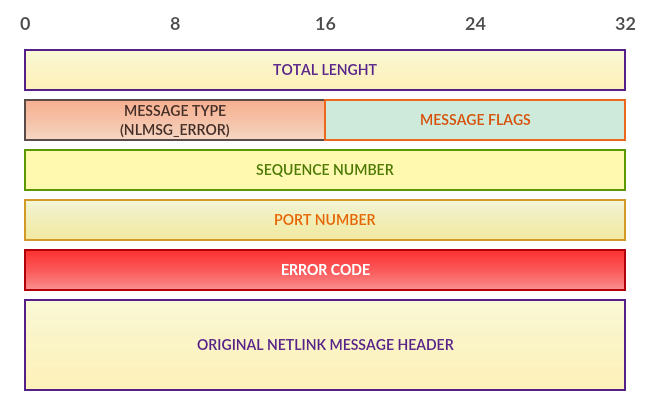
\includegraphics[width=10cm]{nlmsgerror}%inserisce una figura larga 5cm
                                        %se si vuole usare va scommentata
%
%%%%%%%%%%%%%%%%%%%%%%%%%%%%%%%%%%%%%%%%%inserisce la legenda ed etichetta
                                        %   la figura con \label{fig:prima}
\caption[struct nlmserror]{schema della struttura per il messaggio di risposta}\label{fig:nlmserror}
\end{center}
\end{figure}
VSNLib \`e un progetto in fase di sviluppo scritto in C e completamente opensource, liberamente scaricabile attraverso la piattaforma github al seguente link \url{https://github.com/simonepreite/vsnlib}.

\subsection{Ambiente di Sperimentazione}
Per poter sperimentare e valutare le funzionalita' della libreria VSNLib \`e necessario intercettare le comunicazioni Netlink fra i processi e il kernel.
Per farlo si \`e reso necessario intercettare la system call di invio della richiesta contenente il payload; ovvero l'esecuzione della sendto, verso il socket netlink sotto la nostra attenzione, contenente il buffer della richiesta.\\
In questo punto interviene la nostra libreria che si interpone e, di fatto, fa le veci del kernel, al quale il pacchetto netlink non arriver\`a mai realmente.\\
In partenza VSNLib utilizzava come motore di cattura delle system call la libreria purelibc\cite{K8}, in seguito per\`o si \`e giunti alla conclusione che costruire un modulo ad hoc all'interno del sistema vuos fosse un'alternativa pi\`u versatile, immediata e pulita, inoltre vuos ha un sistema di debug built in che rende pi\`u semplice l'individuazione dei problemi legati allo sviluppo.\\
Vuos\cite{K5} \`e un progetto di virtualsquare, ha come obiettivo quello di virtualizzare parti del sistema operativo senza negare all'utilizzatore la scelta degli elementi da virtualizzare, \`e costruito con un sistema di moduli che possono essere aggiunti a discrezione dell'utente.\\
La versione di sviluppo ufficiale \`e liberamente scaricabile attraverso la piattaforma github al seguente link \url{https://github.com/virtualsquare/vuos}. \\
Per il testing \`e stato creato un fork di vuos contenente il modulo relativo alla cattura delle system call di interesse per VSNLib, anche questa versione reperibile risiede su github \url{https://github.com/simonepreite/vuos}.\\
Il modulo in questione si chiama unrealvsnlib per analogia alla libreria ma ognuno \`e libero di costruire un proprio modulo che si adatti alle esigenze di sviluppo personali.\\

\subsection{Schema}
La libreria costituisce uno strato  intermedio di compatibilit\`a tra netlink e le specifiche configurazioni degli stack.\\
Vediamo come \`e composta:
\begin{description}                     %crea un elenco descrittivo
  \item[VSNLib:] Il primo strato si occupa di inizializzare la libreria in base allo stack che si intende utilizzare (informazione richiesta all'utente) e di mediare la comunicazione tra netlink ed il modulo scelto.\\
  Indicare esplicitamente il modulo desiderato \`e una scelta implementativa dettata dal principio di avere un core che sia il pi\`u contenuto possibile.
  \item[Modules:] Sono la parte specifica della libreria, essi contengono l'intestazione delle funzioni generiche che si occupano di chiamare quelle particolari per ogni stack.
\end{description}
\begin{figure}[h]                       %crea l'ambiente figura; [h] sta
                                        %   per here, cio� la figura va qui
\begin{center}                          %centra nel mezzo della pagina
                                        %   la figura
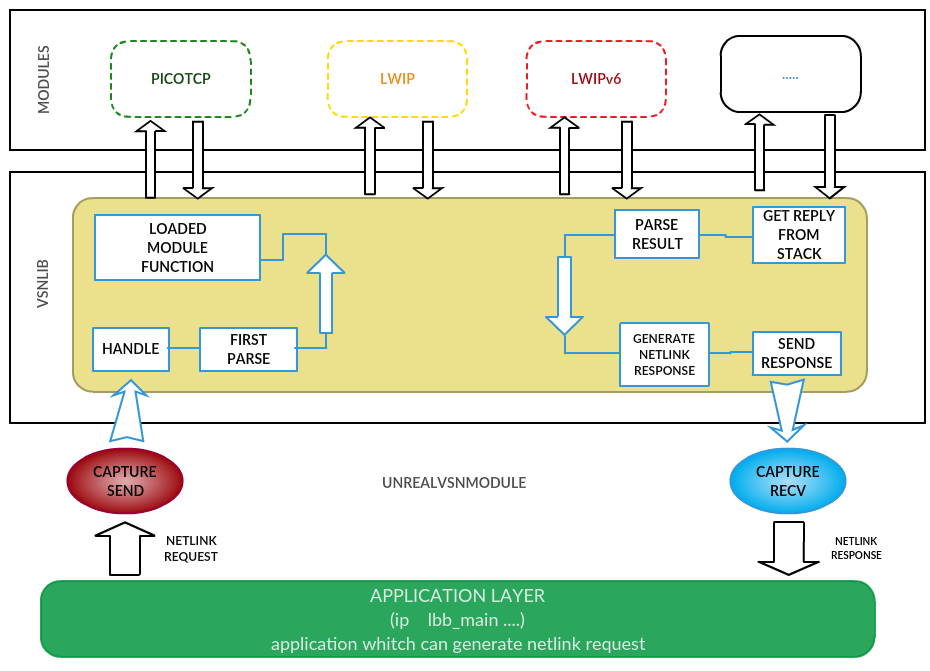
\includegraphics[width=14cm]{vsnlib_scheme}%inserisce una figura larga 5cm
                                        %se si vuole usare va scommentata
%
%%%%%%%%%%%%%%%%%%%%%%%%%%%%%%%%%%%%%%%%%inserisce la legenda ed etichetta
                                        %   la figura con \label{fig:prima}
\caption[mappa concettuale libreria]{mappa concettuale libreria}\label{fig:map}
\end{center}
\end{figure}
\subsection{VSNLib}
Espone le interfacce di comunicazione della libreria, che di fatto sono due, una per inizializzare l'ambiente ed una per inviare il pacchetto da gestire.\\
\begin{lstlisting}[style=CStyle]
int init_vsnlib(char* stack);
void handle_vsnlib(void* buf, size_t len, void* nif, void* stack);
\end{lstlisting}
La prima funzione \`e di inizializzazione della libreria e tramite dlopen ed il nome del modulo da caricare si incarica di popolare l'array di puntatori con i corrispettivi delle funzioni nel modulo.\\
La seconda funzione contiene un loop che cicla sui messaggi del paccheto netlink, che di fatto potrebbero essere pi\`u di uno. Per ogni messaggio ne viene analizzata la tipologia ed in base al tipo si accede all'elemento dell'array che contiene il puntatore alla funzione adeguata a svolgere quel compito.\\
L'utente non ha accesso ad altre funzioni perch\'e \`e la libreria stessa ad analizzare il pacchetto, riempire i campi della struttura generica ed inviarlo al modulo relspecifico dello stack.\\
In risposta si ricever\`a una struttura adatta alla costruzione del paccehetto netlink da spedire alla system call recvfrom del programma in attesa, questo \`e l'ultimo compito della nostra libreria.
\subsection{Moduli}
La presenza di moduli per gestire i vari stack lascia la libert\`a a chiunque necessiti di uno stack non supportato, o personalizzato, di creare il proprio modulo rispettando le specifiche della libreria.\\
Ogni modulo, infatti, ha la stessa struttura e contiene azioni generiche comuni in tutti gli stack. Possiamo vedere i prototipi di una di queste funzioni qui di seguito.
\begin{lstlisting}[style=CStyle]
struct response* adddeladdr(struct config* cfg);
struct response* getaddr(struct config* cfg);
struct response* adddellink(struct config* cfg);
struct response* getsetlink(struct config* cfg);
struct response* adddelroute(struct config* cfg);
struct response* getroute(struct config* cfg);
\end{lstlisting}
In breve ogni modulo \`e composto dallo stesso numero di funzioni che si occupano di mediare la comunicazione tra la libreria e il vero stack.
Ognuna di queste ha un'implementazione diversa a seconda del modulo.\\
Grazie alla tecnica dei puntatori a funzione, si riesce ad essere abbastanza generali e possiamo evitare di specificarne il nome completo.\\
L'idea \`e stata quella di inizializzare, in fase di caricamento della libreria (che avviene con dlopen), un array di puntatori a funzione (attraverso dlsym) in modo tale da poter effettuare le chiamate attraverso di esso. Dlopen e dlsym permettono di caricare dinamicamente solo il modulo di cui si necessita.\\
All' interno dei moduli le funzioni ricevono in input lo stesso tipo di struttura. Durante l'esecuzione di un'azione loro compito \`e la raccola di informazioni dalle funzioni reali dello stack che verranno poi usate per riempire i campi della struttura di risposta che a sua volta servir\`a a creare il payload per il pacchetto netlink di risposta.
%%%%%%%%%%%%%%%%%%%%%%%%%%%%%%%%%%%%%%%%%non numera l'ultima pagina sinistra
\clearpage{\pagestyle{empty}\cleardoublepage}
